A web foi criada para possibilitar o acesso, intercâmbio e recuperação
de informações de maneira rápida e simples, seu crescimento exponencial
e caótico fez com que a mesma se tornasse hoje um gigantesco repositório
de documentos, o que dificulta a recuperação de informações. Até o
momento, não existe nenhuma estratégia abrangente e satisfatória para
a indexação de documentos por meio de “motores de busca” que seja
coerente com uma estrutura linguística. \citet{Souza:2004}.

Um exemplo da deficiência da web atual pode ser identificada na busca
realizada pelos sistemas de recuperação de informação, que usam palavras-chave
nas buscas, onde apenas a similaridade e o número de ocorrências de
certas palavras no conteúdo de documentos são levados em consideração
e não a semântica presente naquela informação. \citep{Souza:2004}.

A Web Semântica tem como finalidade estruturar os dados e informações
disponíveis na Web para que tenham significado e que seja computável,
gerando assim um ambiente onde agentes software e usuários possam
trabalhar de maneira cooperativa, está formada por um conjunto de
padrões propostos pelo World Wide Web Consortium \nomenclature{W3C}{World Wide Web Consortium},
na figura \ref{fig:Semantic_Web_History} podem ser observados os
padrões que constituem a Web Semântica e sua relação com os padrões
XML \nomenclature{XML}{Extensible Markup Language}. A interpretação
do significado é uma habilidade inata dos seres humanos, através da
associação dos conceitos que estão no cérebro por meio de estruturas
neurais. Nas maquinas não existe esta habilidade, devido a que um
dado ou informação é um conjunto de caracteres sem associação a conceitos,
a Web Semântica procura determinar métodos para que as maquinas se
aproximem nesta capacidade, atualmente é possível inferir e deduzir
informações, porem não deve confundir-se com a compreensão humana.

Uma das contribuições da Web Semântica foi a formalização das ontologias,
as quais vão se definir neste capitulo, nas ontologias desenvolvidas
foram modelados os conceitos envolvidos no processo de avaliação da
sustentabilidade em agricultura, definindo, classificando e relacionando
cada um dos conceitos para assim permitir o uso em outros sistemas
e conseguir fazer inferência de novo conhecimento.

Neste capítulo, vamos apresentar e discutir os conceitos usados da
web semântica, exatamente: fundamentos da Web Semântica, Ontologias,
o \foreignlanguage{english}{Resource Description Framework} \nomenclature{RDF}{Resource Description Framework}
e a \foreignlanguage{english}{Web Ontology Language} \nomenclature{OWL}{Web Ontology Language}.

\begin{figure}
\begin{centering}
\includegraphics[width=1\columnwidth]{\string"/home/john/Desktop/masters-degree-dissertation/figures/Semantic Web History\string".eps}
\par\end{centering}
\caption{História da Web Semântica \label{fig:Semantic_Web_History}}
\end{figure}


\section{Web Semântica.}

\citet{bernerslee2001} propuseram a Web Semântica no 2001, como uma
extensão da Web atual na que é possível vincular conceitos de maneira
estruturada e padronizada com a finalidade de gerar uma web universal
dos conhecimentos da humanidade; permitindo assim fornecer conhecimento
estruturado para que seja computável pelas maquinas, e gerar um meio
comum de representação entre os humanos e maquinas.

A partir desta visão conceitual sobre a Web, Berners-Lee propôs uma
arquitetura que organiza as representações do conhecimento por meio
de camadas, dita arquitetura é conhecida como \foreignlanguage{english}{Semantic
Web Cake} que é ilustrada na Figura \ref{fig:Web-Semantic-Architecture}

\begin{figure}
\caption{Arquitetura em camadas da Web Semântica\label{fig:Web-Semantic-Architecture}}
\includegraphics{\string"/home/john/Desktop/masters-degree-dissertation/figures/Semantic Web Architecture\string".eps}
\end{figure}

A base da arquitetura é estabelecida pelos padrões \foreignlanguage{english}{Unicode}
e URI, que padronizam a representação dos dados. 

\selectlanguage{english}%
Unicode\foreignlanguage{brazil}{ é um padrão que codifica os caracteres
na maioria dos sistemas de escrita para representação de texto com
fines de processamento computacional.}

\selectlanguage{brazil}%
URI \nomenclature{URI}{Uniform Resource Identifier} permite identificar
unificadamente os recursos disponíveis na Web por meio de uma \foreignlanguage{english}{String.}

A camada \nomenclature{XML}{eXtensible Markup Language} representa
os dados de maneira sintática, através a definição de \foreignlanguage{english}{markups}
os quais codificam os documentos dando formato preestabelecido e permitindo
que as informações sejam legíveis tanto por humanos como por computadores,
suportando as camadas superiores na arquitetura da Web Semântica.

A camada de descrição está representada na especificação \foreignlanguage{english}{\nomenclature{RDF}{eXtensible Markup Language}}
que é usada como um método geral para descrição conceitual o modelagem
de informação por meio de recursos, usa notações sintáticas e formatos
de serialização.

A camada \foreignlanguage{english}{Ontology} estende a camada de descrição,
fornecendo mais expressividade na definição de conceitos, relações
semânticas dos conceitos.

A camada \foreignlanguage{english}{Logic} permite definir regras logicas
para deduzir e inferir novas informações que conseguem mudar a estrutura
da ontologia de maneira dinâmica.

A camada \foreignlanguage{english}{Proof} fornece mecanismos para
avaliar o nível de confiabilidade das fontes de recursos e informações.

A camada \foreignlanguage{english}{Trust} representa o conhecimento
validado e confiável.

O componente \foreignlanguage{english}{Digital Signature} permite
integrar métodos de segurança que garantam a confiabilidade da informação.

O presente trabalho incluiou desde as camadas inferiores até o OWL,
permitindo definir ontologias que representem os domínios de conhecimento.

\section{Ontologias}

\citet{Smith2007} descreve a ontologia como uma área da filosofia,
que estuda a natureza, existência e realidade dos entes, assim como
as categorias do ser e das relações semânticas.

\citet{allemang2011semantic} define as ontologias no contexto da
Web Semântica como um esquema de representação que permite conceitualizar
e estruturar conhecimento, permitindo a interpretação dele através
das computadoras, cujo principal objetivo é compartilhar conhecimento
entre humanos e computadoras.

Na ciências da computação e informação, a palavra ``ontologia''
define-se como uma especificação formal e explicita de uma conceitualização
compartilhada de um domínio de conhecimento.

Segundo \citet{Patel-schneider05buildingthe} a representação de ontologia
é realizada por meio de lógica de predicados e lógica descritiva,
usando padrões adotados pela comunidade como RDF e OWL.

Uma ontologia é um sistema de organização e representação do conhecimento,
em inglês\emph{ }\foreignlanguage{english}{\emph{Knowledge Organization
System}} (\emph{KOS\nomenclature{KOS}{Knowledge Organization System}}),
que é uma estrutura conceitual e computacional que permite representar
o conhecimento, de qualquer domínio, por meio de entidades, classificações,
relações semânticas, regras e axiomas.

Uma ontologia é especificada por meio de componentes básicos que são
as classes, relações, axiomas e instâncias. As \textbf{classes}, o
foco da maioria das ontologias, são utilizadas para descrever os conceitos
de um domínio, possibilitando a organização e classificação dos individuos
em um sistema lógico e hierárquico contendo subclasses que representam
conceitos específicos \citet{noy2001ontology}. As \textbf{relações}
representam o tipo de interação entre os conceitos de um domínio e
as propriedades presentes nas classes e indivíduos. Elas podem ter
características próprias, como serem transitivas, simétricas, ou terem
uma cardinalidade definida. Os \textbf{axiomas} são utilizados para
modelar regras assumidas como verdadeiras no domínio em questão, de
modo que seja possível associar o relacionamento entre os indivíduos,
além de fornecer características descritivas e lógicas para os conceitos.
Por fim, os \textbf{indivíduos}, ou instâncias das classes, são utilizados
para representar elementos específicos, ou seja, os próprios dados,
que juntamente com a definição de uma ontologia, constituem a base
de conhecimento \citep{noy2001ontology}. Os indivíduos representam
objetos do domínio de interesse \citet{horridge2011owl}.

A Figura \ref{fig:Smart-data-continuum} mostra os níveis de representação
de dados na forma de conhecimento processável por máquinas.

\begin{figure}[H]
\centering{}\includegraphics[width=0.8\columnwidth]{\string"/home/john/Desktop/masters-degree-dissertation/figures/smart data\string".eps}\caption{\foreignlanguage{english}{Smart data continuum\foreignlanguage{brazil}{: níveis de representação
de dados na forma de conhecimento processável por máquinas.\label{fig:Smart-data-continuum}}}}
\end{figure}

O nível mais baixo de representação começa com os dados sem nenhum
significado semântico, dependentes do contexto da aplicação. O segundo
nível envolve a definição de esquemas XML para conseguir independência
dos dados da aplicação, os dados fluem entre aplicações em um único
domínio mas não podem ser compartilhados fora do domínio. No terceiro
nível, os dados podem ser combinados a partir de diferentes domínios,
sendo suficientemente independentes para serem recuperados e combinados
com outras fontes de dados. Finalmente no quarto nível, é possível
inferir novos dados a partir dos existentes e compartilha-os entre
aplicações sem requerer interferência humana \citep{sugumaran2011},
cada uma destas caraterísticas compõem as ontologias.
\selectlanguage{english}%

\section{Resource Description Framework\foreignlanguage{brazil}{ (RDF)}}

\selectlanguage{brazil}%
O \foreignlanguage{english}{\nomenclature{Resource Description Framework}{RDF}}
é uma família de especificações da W3C, que foi disponibilizada em
1999 como parte do W3C's \foreignlanguage{english}{Semantic Web Effort},
que fornece um \foreignlanguage{english}{Framework} comum que permite
aos dados ser compartilhados e reusados através das fronteiras das
aplicações, empresas e comunidades \footnote{http://www.w3.org/2001/sw/}.
Ele foi originalmente projetado como um modelo de meta-dados e também
chegou a ser usado como um método de descrições conceituais, principalmente
para descrever recursos web. 

O RDF é usado em várias áreas de aplicação, como \foreignlanguage{english}{\emph{resource
discovery}} para melhorar as capacidades dos motores de busca, \foreignlanguage{english}{\emph{cataloging}}
para descrever o conteúdo e as relações de conteúdo disponibilizados
em um sistema web particular e descrição de \foreignlanguage{english}{\emph{intellectual
property rights}} de páginas web.

O modelo básico de dados consiste em um padrão de três tipos de objetos:
\begin{itemize}
\item Sujeito: representa os recursos e são identificados por meio de URIs,
sem importar o tamanho deles, por exemplo, uma pagina web ou um elemento
\nomenclature{HTML}{HyperText Markup Language} podem ser recursos.
\item Predicado: são aspectos, características, atributos ou relações especificas
que descrevem o sujeito, cada predicado têm um significado especifico
e relaciona um sujeito com um objeto.
\item Objeto: um recurso especifico ou valor da propriedade que representa
uma características do objeto \footnote{http://www.w3.org/TR/PR-rdf-syntax/}
\end{itemize}
Com RDF é possível explicitar relações entre dois objetos (usando-se
uma Tripla RDF), mas não consegue fazer modelagens especificas nem
integrar inferência. Para se descrever o que um objeto representa
e suas relações com outros objetos, são necessárias ontologias. 

\section{Web Ontology Language (OWL)}

A \foreignlanguage{english}{Web Ontology Language} (OWL) foi recomendada
pelo W3C em 2004 para representar e compartilhar ontologias na Web.
Essa linguagem foi projetada para aplicações que necessitam processar
o conteúdo da informação em vez de apenas apresentar informações em
nós \citet{mcguinness2004owl}. OWL é uma linguagem que permite que
a semântica seja explicitamente associada ao conteúdo dos dados na
web e formalmente especificada através de ontologias, compartilhadas
na Internet. 

A versão OWL 2 é a versão mais recente da linguagem OWL. De acordo
com as especificações do W3C\footnote{http://www.w3.org/TR/owl2-overview/},
a OWL 2 adicionou três novos perfis (sub-linguagens) aos perfis DL
e Full já existentes: OWL 2 EL, OWL 2 QL e OWL RL (Figura \ref{fig:OWL2-Profiles}).
Cada um desses perfis oferece um poder de expressividade diferente
para diversos cenários de aplicação:
\begin{description}
\item [{Full}] O perfil OWL Full é direcionado para usuários que querem
a máxima expressividade e a liberdade sintática do RDF sem nenhuma
garantia computacional. É improvável que qualquer software de raciocínio
seja capaz de suportar completamente cada recurso da OWL Full \citep{mcguinness2004owl}.
\item [{DL}] O perfil OWL DL (\foreignlanguage{english}{Description Logic})
é para aplicações que necessitam de máxima expressividade, enquanto
mantém a computabilidade (todas as conclusões são garantidos para
ser computáveis) e decidibilidade (todas as computações terminarão
em tempo finito) \citep{mcguinness2004owl}. OWL DL inclui todas as
construções da linguagem OWL, mas elas podem ser usadas somente sob
certas restrições. 
\item [{EL}] O perfil OWL 2 EL é baseado na família EL++ de lógica descritiva
(\foreignlanguage{english}{Description} \foreignlanguage{english}{Logic}),
esse perfil é particularmente útil em aplicações utilizando ontologias
que contêm um grande número de propriedades e/ou classes. Além disso,
o OWL 2 EL utiliza um padrão comum utilizado em ontologias para conceitos
e planejamento, ou seja, a combinação de conjunção e qualidades existenciais.
\item [{QL}] O perfil OWL 2 QL é baseado na família DL-Lite de lógica descritiva.
Esse perfil foi criado para permitir o raciocínio (\foreignlanguage{english}{reasoning})
eficiente com grandes quantidades de dados estruturados de acordo
com esquemas relativamente simples. Ele fornece a maioria dos recursos
necessários para capturar modelos conceituais, tais como diagramas
de classe UML, diagramas de Entidade de Relacionamento, e esquemas
de banco de dados. 
\item [{RL}] O perfil OWL 2 RL é voltado para aplicações que exigem raciocínio
escalável em troca de alguma restrição de poder expressivo. Ele define
um subconjunto sintático de OWL 2 que favorece a implementação utilizando
tecnologias baseadas em regras. Esse perfil pode ser utilizado na
maioria das construções OWL 2, porém, para permitir implementações
baseadas em regras de raciocínio, a forma como essas construções podem
ser usadas em axiomas foi restringida. 
\end{description}
\begin{figure}[H]
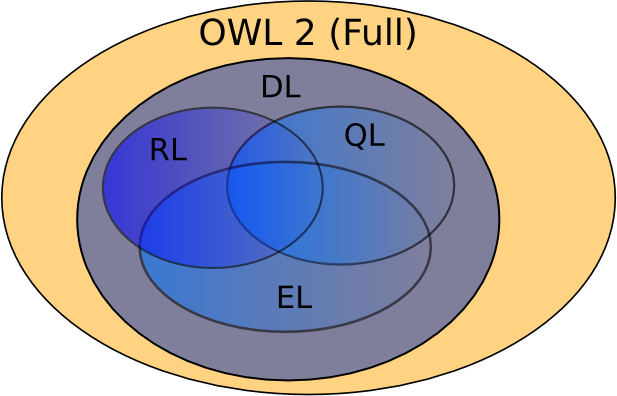
\includegraphics[width=0.8\columnwidth]{/home/john/Desktop/masters-degree-dissertation/figures/owl2-profiles}

\caption{OWL2 Profiles.\label{fig:OWL2-Profiles}}
\end{figure}


\section{Considerações finais}

Os conceitos apresentados anteriormente foram necessários para o desenvolvimento
do sistema gerador de SADs, demostrando que a web semântica fornece
o suporte tecnológico e teórico suficiente para abordar o desenvolvimento
de sistemas baseados em conhecimento, particularmente as ontologias
suportaram vários aspectos cruciais no desenvolvimento deste projeto,
pelo qual elas foram o foco central da presente pesquisa. Através
dos conceitos definidos nelas, será possível associar tipos aos dados
e modos de apresentação dos mesmos (por exemplo, tipos de gráficos
de apresentação), a partir dessas descrições, \foreignlanguage{english}{widgets}
podem ser geradas de maneira automática e assim suportar a geração
de SADs de maneira semiautomática.
